\documentclass[aspectratio=169]{beamer}

\usepackage[utf8]{inputenc}
\mode<presentation>
{
  \usetheme{Darmstadt}      % or try Darmstadt, Madrid, Warsaw, ...
  \usecolortheme{beaver} % or try albatross, beaver, crane, ...
  \usefonttheme{serif}  % or try serif, structurebold, ...
  \setbeamertemplate{navigation symbols}{}
  \setbeamertemplate{caption}[numbered]
  \setbeamertemplate{footline}[frame number]
  \setbeamertemplate{headline}{}
} 
\usepackage{graphicx}
\usepackage[english]{babel}
\usepackage[utf8]{inputenc}
\usepackage[T1]{fontenc}
\usepackage{bm}
\usepackage{amssymb}
\usepackage{amsmath}
\usepackage{bm}
\usepackage{leftidx}
\usepackage{mathtools}
\usepackage{tikz}
\usepackage{gensymb}
\usepackage{listings}
\pdfsuppresswarningpagegroup=1

\begin{document}
\AtBeginSection[]{
  \begin{frame}
  \vfill
  \centering
  \begin{beamercolorbox}[sep=8pt,center,shadow=true,rounded=true]{title}
    \usebeamerfont{title}\insertsectionhead\par%
  \end{beamercolorbox}
  \vfill
  \end{frame}
}

\title[Your Short Title]{Control of a Hurricane Hunting Aircraft}
\author{Corey Spohn, Jacob Pelster, Rachel Oliver, and Zvonimir Stojanovski}
\institute{MAE 6780 Multivariable Control Theory}
\date{\today}

\begin{frame}
  \titlepage
\end{frame}

\begin{frame}{Model Predictive and Sliding Mode Control}
    \begin{columns}
        \begin{column}{0.5\textwidth}
            Model Predictive Control
            \begin{itemize}
                \item Quadratic cost function with a finite horizon
                \begin{eqnarray*}
                J = & \int_0^{T_{p}} \! [\mathbf{x}(t_{i}+\tau|t_{i})^T\mathbf{Q}\mathbf{x}(t_{i}+\tau|t_{i}) \\ &  +\Dot{\mathbf{u}}(\tau)^T\mathbf{R}\Dot{\mathbf{u}}(\tau)] \, \mathrm{d}\tau
                \end{eqnarray*}
                \item Incremental control implementation\\
                    $ \mathbf{u}(t\rightarrow{t+1}) = -\mathbf{K}_{mpc}*\mathbf{x}(t)$
            \end{itemize}
            \begin{figure}
                \centering
                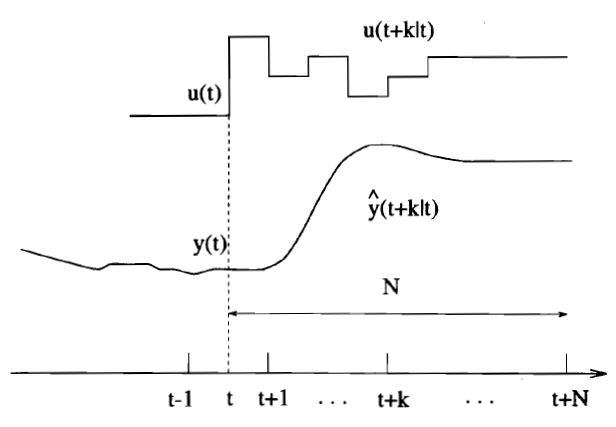
\includegraphics[width=0.6\textwidth]{MPC_Premise.PNG}
            \end{figure}
        \end{column}
        \begin{column}{0.5\textwidth}
            Sliding Mode Control
            \begin{itemize}
                \item Want to confine state $\mathbf{x}$ to surface $\boldsymbol{\sigma}(\mathbf{x})=\mathbf{0}$ (``sliding surface'') on which system is stable
                \item Control proportional to $\mathrm{sgn}(\boldsymbol{\sigma})$ brings state to sliding surface in finite time (but often better to use sigmoid function to avoid ``chatter'')
                \item Stability conditions depend only on bounds of system dynamics
                \item Can be combined with Model Predictive Control
            \end{itemize}
        \end{column}
    \end{columns}
\end{frame}

\begin{frame}{Preliminary Results}
    \begin{columns}
        \begin{column}{0.5\textwidth}
            Model Predictive Control
            \begin{figure}
                \centering
                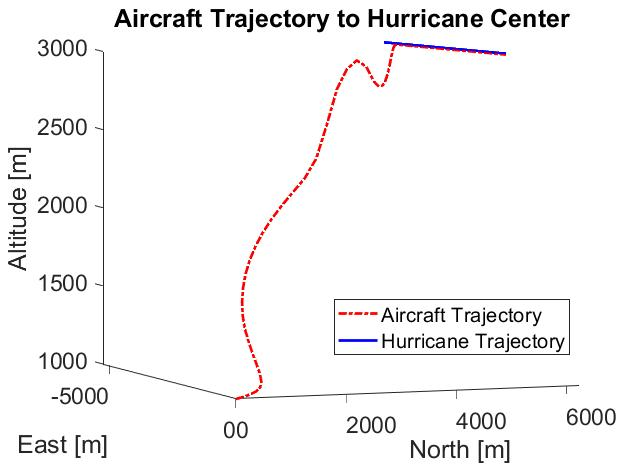
\includegraphics[width=.6\textwidth]{Prelim_MPC_Results.jpg}
            \end{figure}
            \begin{figure}
                \centering
             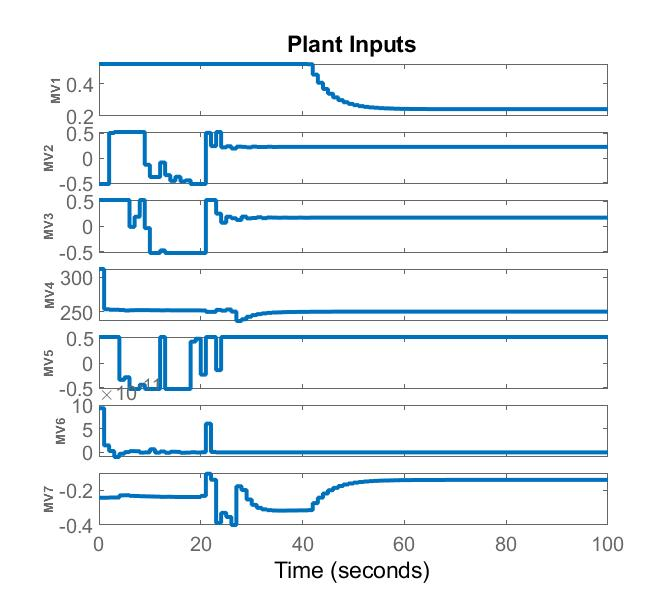
\includegraphics[width=.55\textwidth]{Prelim_MPC_Inputs.jpg}
            \end{figure}
        \end{column}
        \begin{column}{0.5\textwidth}
            Sliding Mode Control
            \begin{figure}
                \centering
                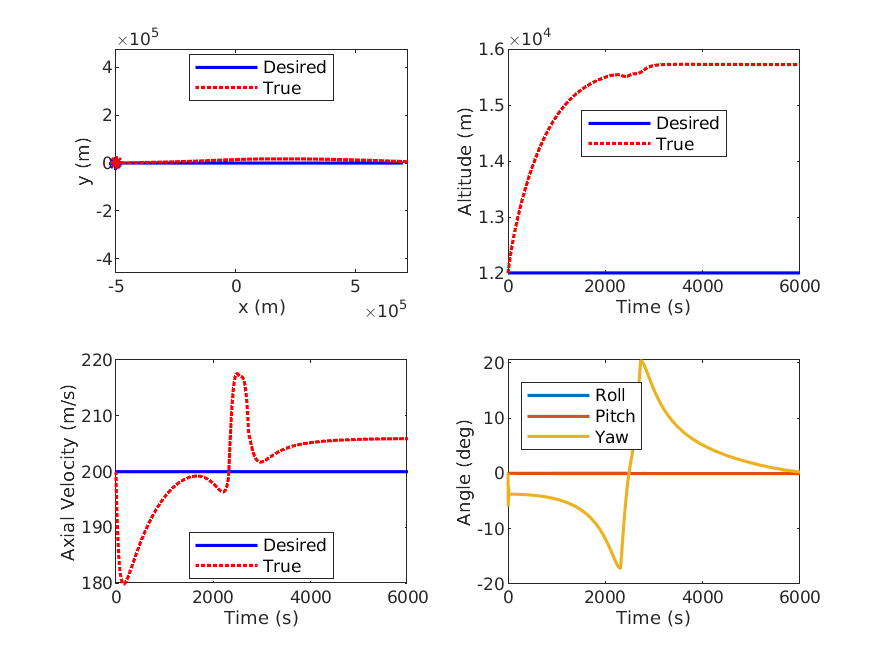
\includegraphics[width=1\textwidth]{sm_flight.png}
            \end{figure}
        \end{column}
    \end{columns}
\end{frame}

\begin{frame}{The Way Ahead}
    \begin{itemize}
        \item Adjust wind field to have a radial velocity, $V_r$, that varies by radius, $r$, from hurricane center to plant, example below taken from Kalourazi 2020.
        \begin{columns}
        \begin{column}{0.7\textwidth}
            \begin{align}
            V_r = 
            \begin{cases}
                    V_{max} \left( \frac{r}{R_{max}}\right)^{\frac{3}{2}}, & r < R_{max} \\
                    V_{max} \left( \frac{2 R_{max} r}{r^2 + R_{max}^2} \right), & r \geq R_{max} 
            \end{cases}
            \end{align}
            \end{column}
            \begin{column}{0.3\textwidth}
                \begin{figure}
                \centering
                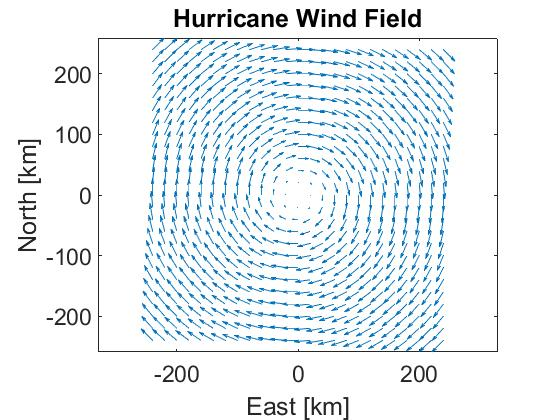
\includegraphics[width=1\textwidth]{HurricaneWindField.jpg}
            \end{figure}
            \end{column}
        \end{columns}
        
        \item Decrease chattering while allowing for constraints by combining sliding mode and MPC
        \item Try more challenging sampling missions by maintaining steady level flight in hurricane regions
        \item Comparison of flight trajectories and input requirements when prioritizing energy savings
    \end{itemize}
\end{frame}

\begin{frame}{References}
    \nocite{*}
    \footnotesize
    \bibliographystyle{ieeetr}
    \bibliography{references}
\end{frame}

\end{document}